\section{Nonlinear Regression}
\subsection{Prior Works}
\begin{frame}{Approximation Method}
  \begin{itemize}
    \item Canonical Hemodynamic Response Function
    \begin{itemize}
        \item No Parameters Estimated
        \item Maximum Likelihood Possible
        \item Inflexible - even to changes in onset time
    \end{itemize}
    \item 2nd Order Volterra Kernel \cite{Friston2000}
    \begin{itemize}
        \item Quadratic Convolution used to approximate Jacobian Matrix.
        \item Volterra approximation quality is not known.
    \end{itemize}
    {\footnotesize
    $$y(t) = k_0 + \int_{-\infty}^{\infty} k_1(s_1) x(t-s_1) ds_1
        + \int_{-\infty}^{\infty} k_2(s_1,s_2) x(t-s_1)x(t-s_2) ds_1 ds_2$$
    }
    \begin{center}
    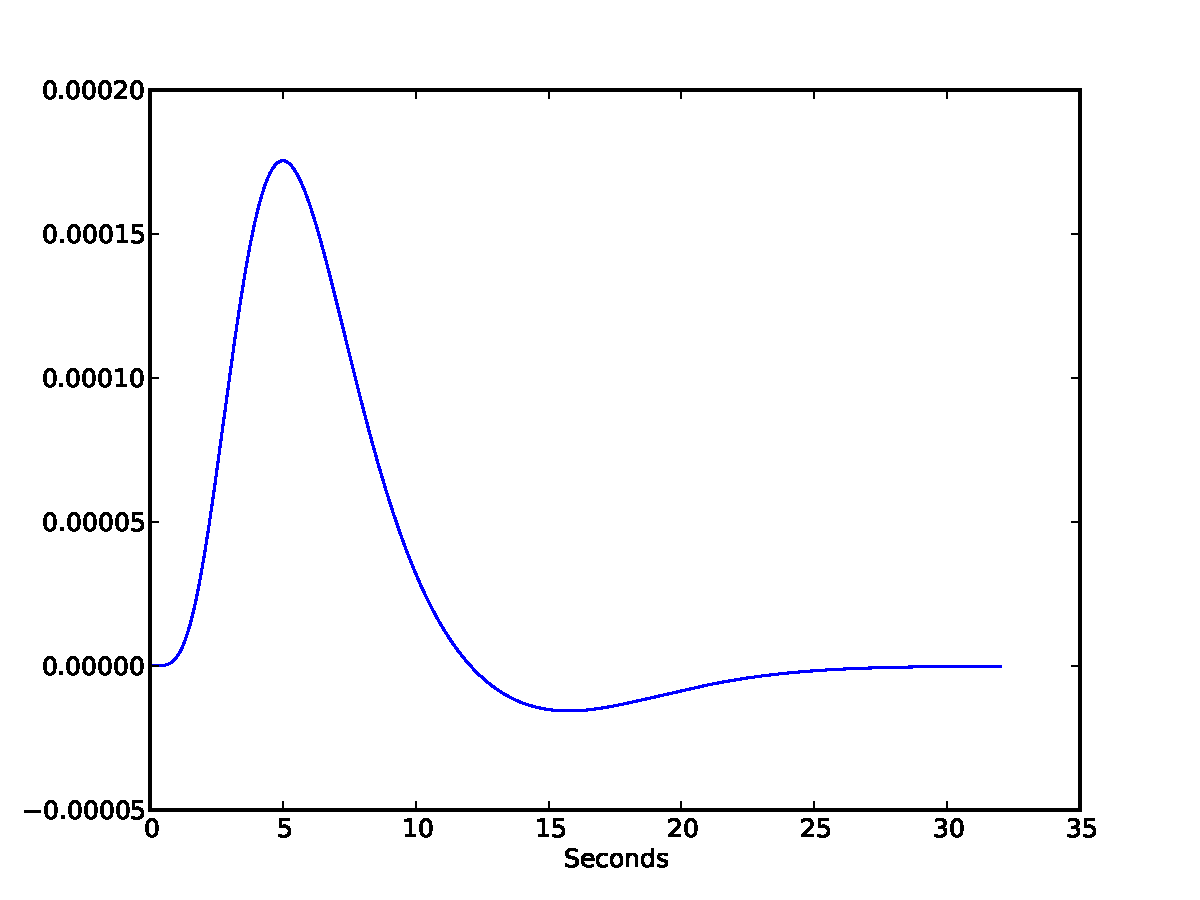
\includegraphics[clip=true,trim=4.88cm 0cm 5cm 1.5cm,height=2.7cm,width=8cm]{HRF}
    \end{center}
    
  \end{itemize}
  \note{
    \begin{itemize}
        \item Neither of these is truly nonlinear method
        \item General Linear Model uses a generic Kernel across all
                regions.
        \item Canonical Hemodynamic Response Function
        \item Fast, Maximum Likelihood, Not Adaptive, same across regions/patients
                pathologies
        \item Volterra Kernel Potentially Offers a Better Fit
        \item If Kernels Could be quickly optimized, it could work
        \item Never really used, because optimizing kernels is slow, and
                its still an approximation
    \end{itemize}
  }
\end{frame}

\begin{frame}{Nonlinear Methods}
\begin{itemize}
    \begin{columns}
    \begin{column}{.45\textwidth}
    \item Local Linearization filter, \cite{Riera2003}
    $$f(t)- f(t-1) \sim N(0, \sigma^2)$$
    \item Genetic Algorithms and Simulated Annealing, \cite{Vakorin2007}
    \item Unscented Kalman Filter \cite{Hu2009}
    \item Particle Filters to estimate States, \cite{Murray2009}
    \begin{itemize}
        \item ML estimate of $\Theta$, \cite{Johnston2007}
    \end{itemize}
    \end{column}

    \begin{column}{.55\textwidth}
    \begin{figure}
    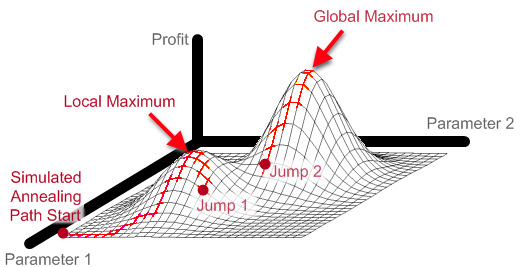
\includegraphics[clip=true,trim=0cm 0cm 0cm 1cm,width=.6\textwidth]{simulated_annealing}
    \caption{Simulated Annealing can escape local minima with chaotic jumps. \cite{Dama}}
    \end{figure}
    \begin{figure}
    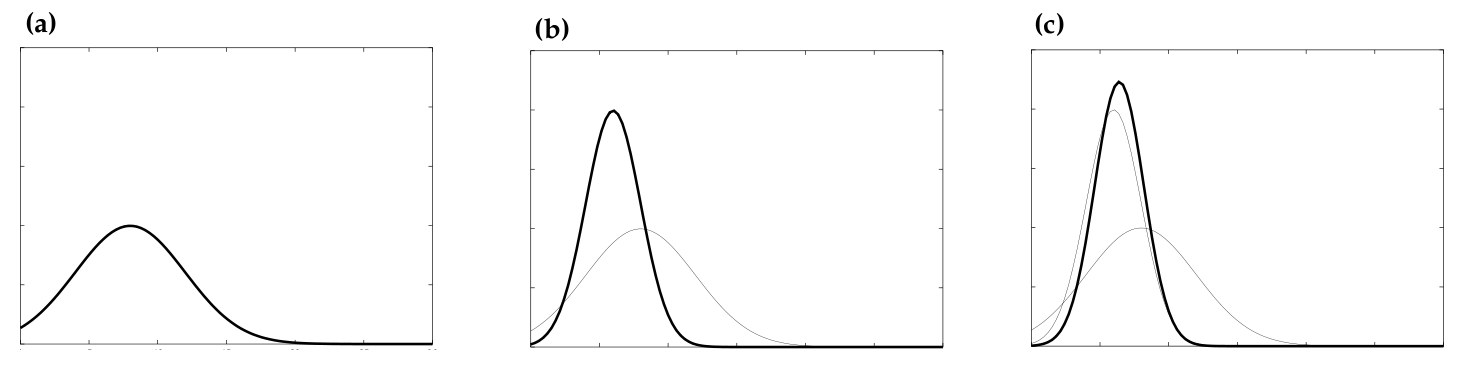
\includegraphics[width=\textwidth]{kalman}
    \caption{UKF: (a) Initial Belief  (b) Noisy Measurement  (c) incorporated into the belief. \cite{Thrun2005}}
    \end{figure}
    \end{column}
    \end{columns}
\end{itemize}
\note{
    \tiny
    \begin{itemize}
     \item Riera: Local Linearize
        \begin{itemize}
            \tiny
            \item Compare Estimated Step (Adjacent Measurements) With Actual Step
            \item Jacobian is available - gradient descent possible
            \item Removes Drift/Structured Noise
            \item Completely Removes DC component - 
            \item Quality Depends on experimental design: less Effective For 
                    Block Stimulus
        \end{itemize}
        \item Vakorin: GA used to optimize spike train, Simulated Annealing 
            to Estimate Parameters
        \item Simulated Annealing is Slow, every step: BOLD recalc
        \item UKF linearizes the noise, propagates limited number of 
                samples through the state equation, and then uses 
                first 2 moments
        \item Murray kept parameters constant, all differences result of 
            state-noise
        \item Johnston - used estimated state distribution to perform
                maximum likelihood on other parameters.
        \item ($P(X, \Theta | Y) = P(X | Y, \Theta) P(\Theta | Y)$)
        \item Johnston's Results don't mesh
        \item Neither of previous particle filter methods considered it
                possible 
        \item All of these methods focus on point estimate of the solution
    \end{itemize}
}
\end{frame}

\subsection{Particle Filter}
%frame with example
\begin{frame}{Example System Identification}
\begin{itemize}
\item Given:
    \begin{itemize}
    \item Elevation Map (1D)
    \item Ability To Measure Elevation
    \end{itemize}
\item Particle Consists of the unknowns:
    \begin{itemize}
    \item State: Location  $[0, 20]$
    \item Constant: Direction  $\{Left, Right\}$
    \end{itemize}
\end{itemize}

\begin{center}
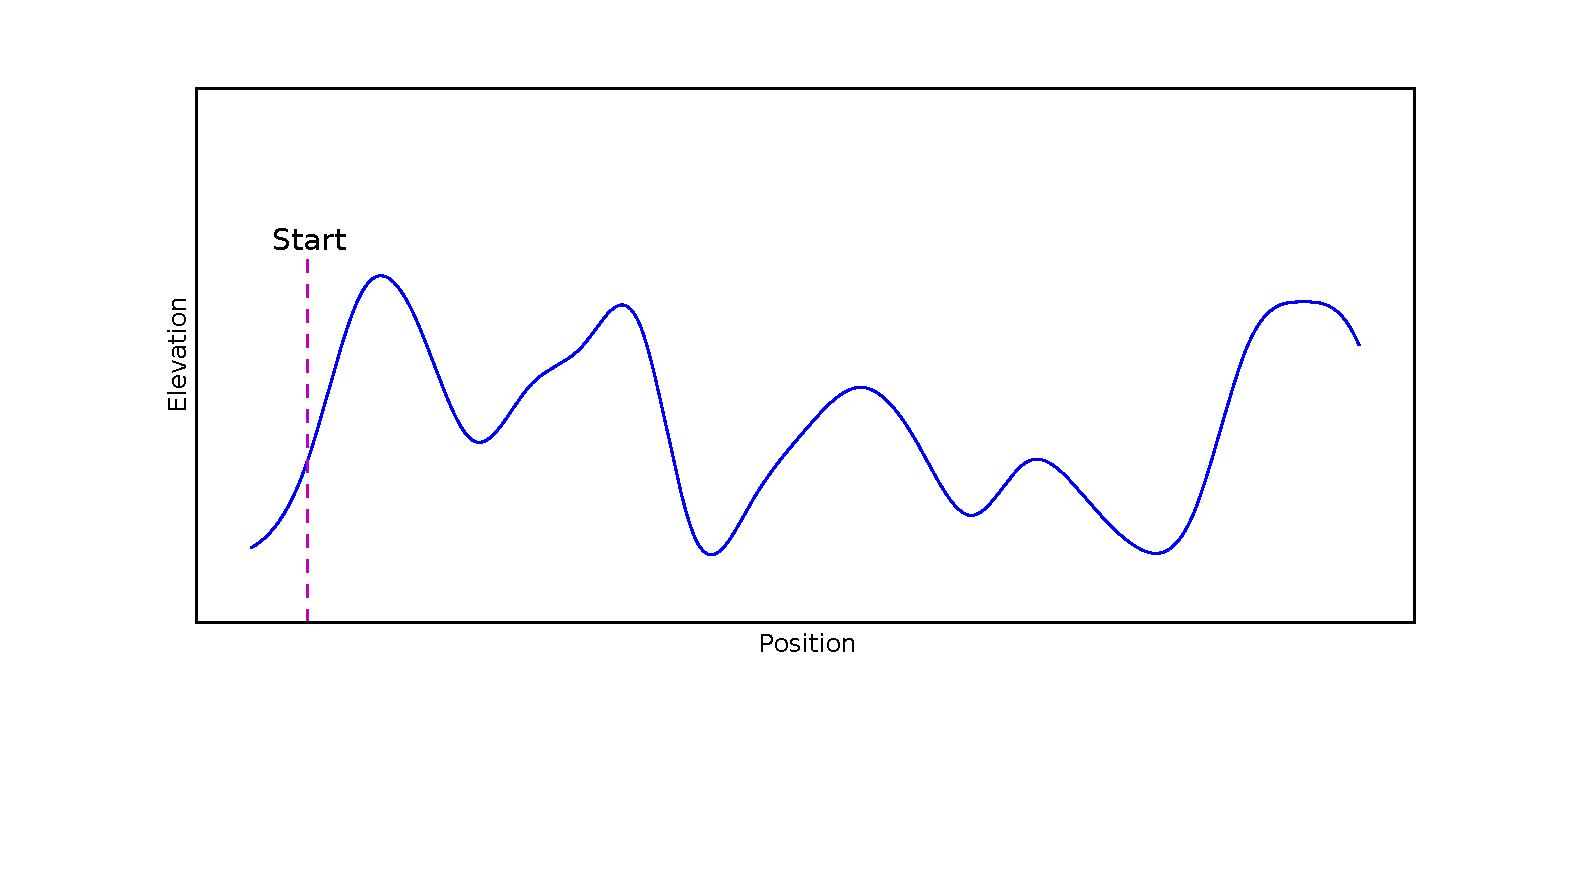
\includegraphics[clip=true,trim=2cm 3cm 3cm 3cm,width=.7\textwidth]{setup}
\end{center}
\note{
\begin{itemize}
    \item Start with an example.
    \item One dimensional mountain range
    \item Have a map and an altimeter to measure elevation
    \item Don't know where you are or which direction you are moving
    \item Need a prior distribution that spans both dims direction/location
\end{itemize}
}
\end{frame}

\begin{frame}{Initial Distribution}
\centering
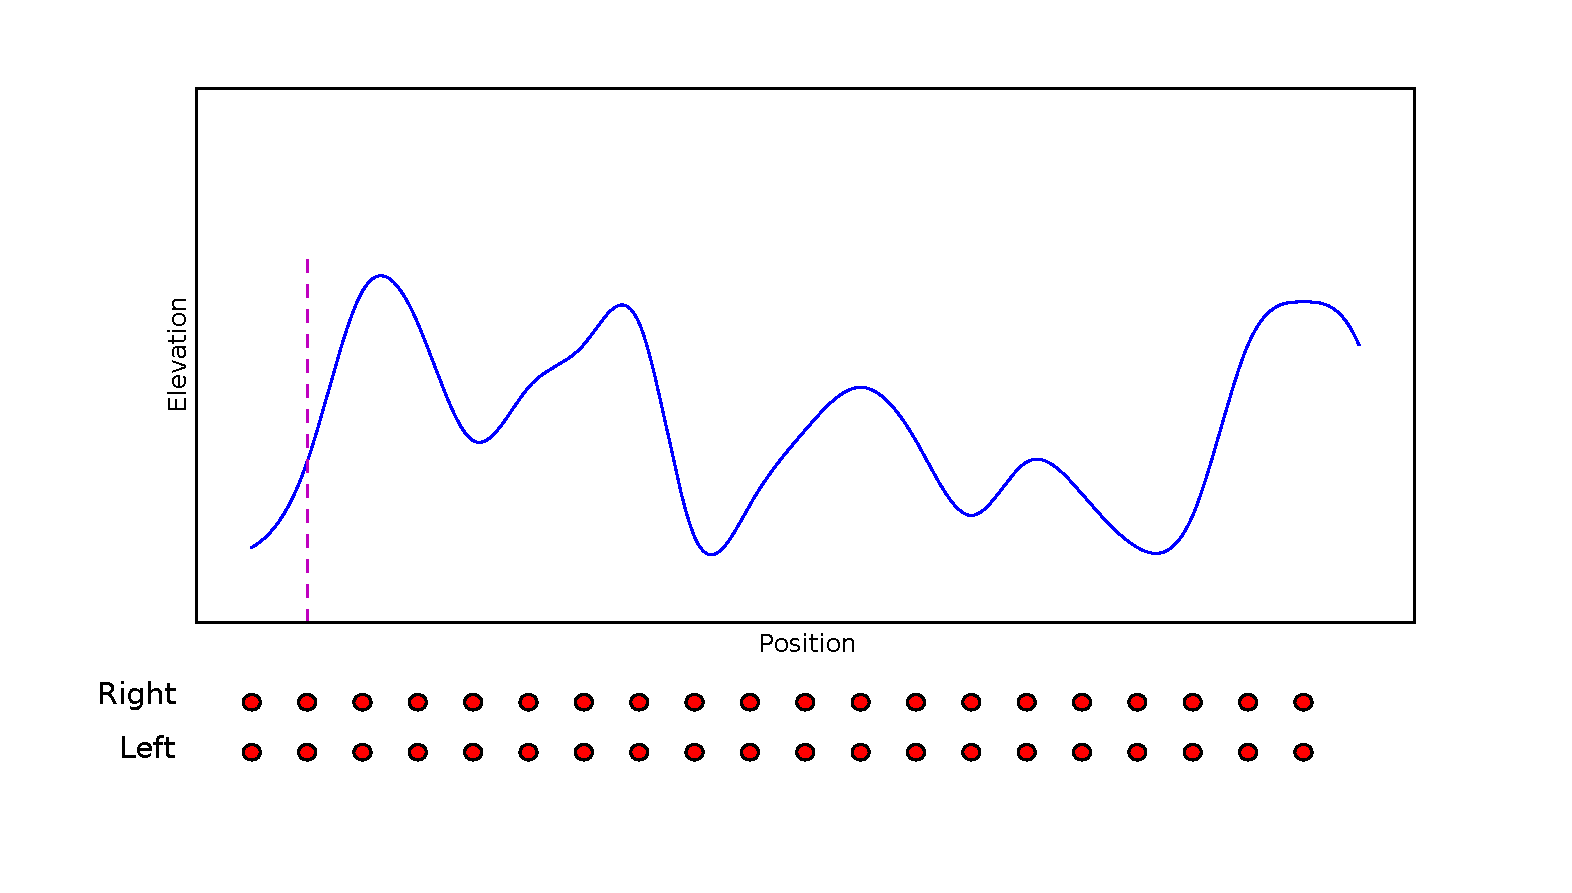
\includegraphics[width=\textwidth]{init}
\note{
\begin{itemize}
    \item Here is the prior, 20 locations, either right or left, 
        40 total particles
    \item So each particle contains a unique direction and position
\end{itemize}
}

\end{frame}

\begin{frame}{Measurement 1}
\centering
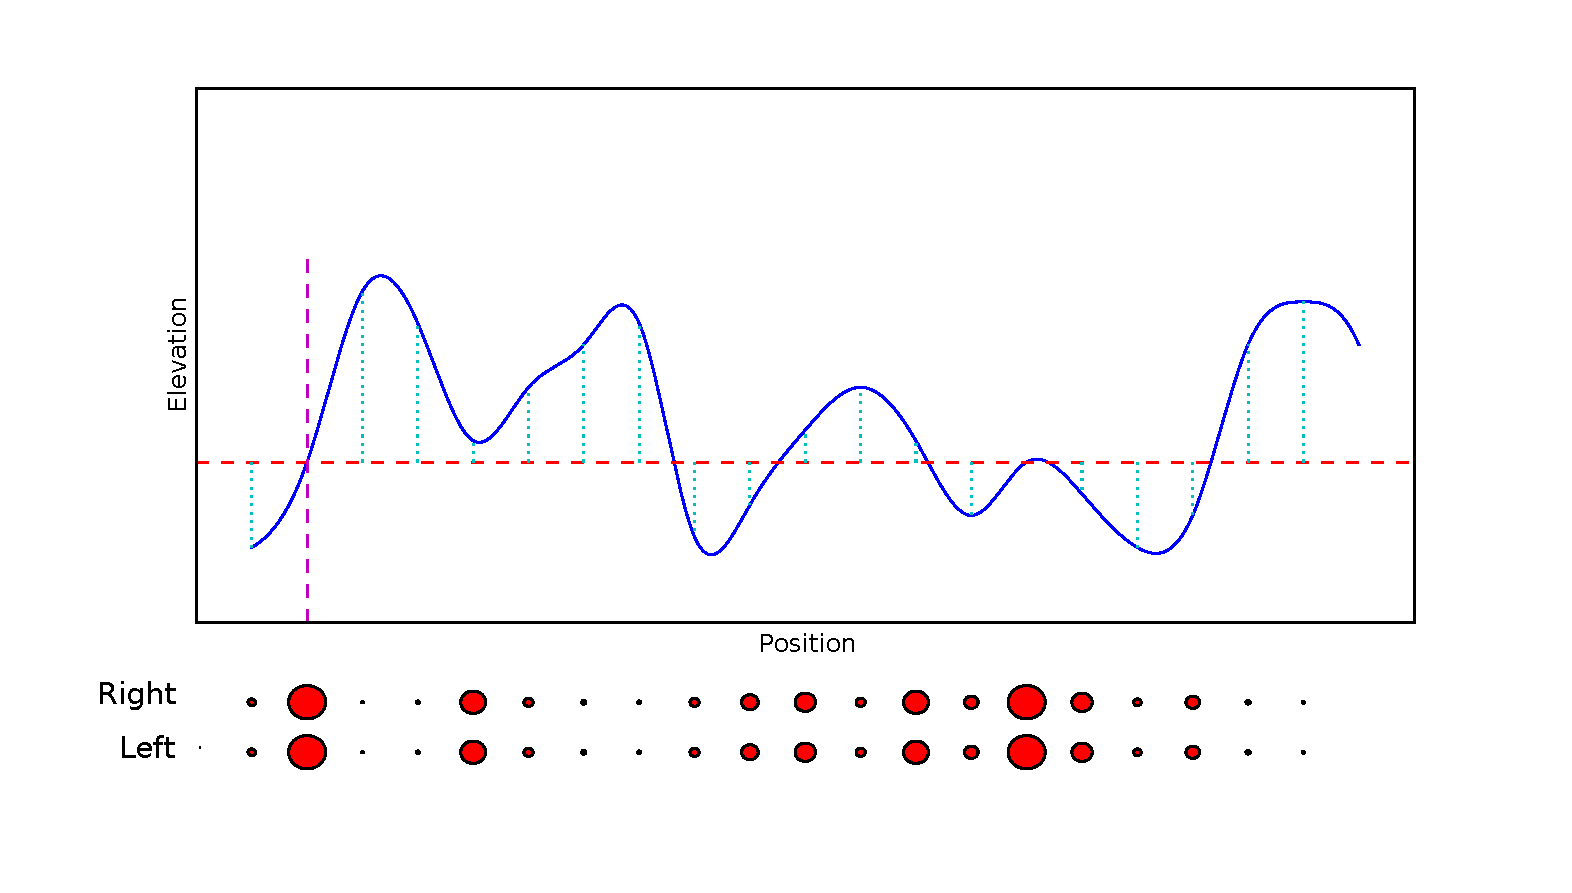
\includegraphics[width=\textwidth]{meas1}
\note{
\begin{itemize}
    \item Now measure the elevation, and weight locations that are close
            to that elevation higher
    \item Note the second downhill, No particles nearby in terms of $\Delta y$.
    \item Compare that to the next uphill
    \item Relation between particle spacing and weighting function
    \item Now we've applied a measurement, now need to integrate state
            until the next measurement becomes available.
\end{itemize}
}
\end{frame}

\begin{frame}{Step Forward}
\centering
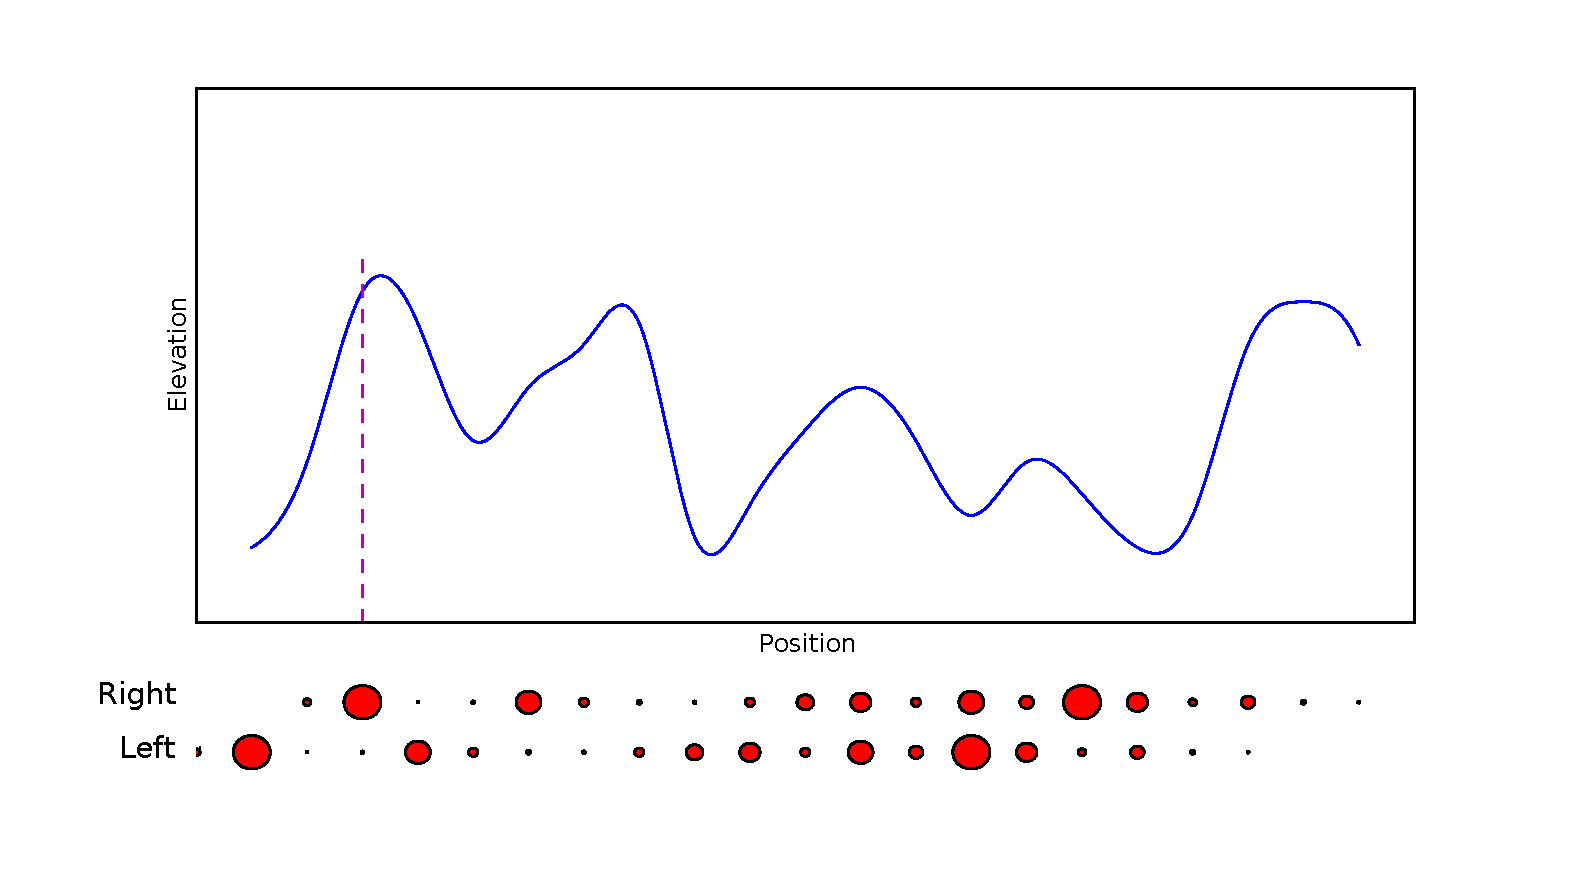
\includegraphics[width=\textwidth]{move1}
\note{
    \begin{itemize}
    \item Notice that no movement occurs in terms of right/left. Those
            are parameters and so they don't change with time.
    \end{itemize}
}
\end{frame}

\begin{frame}{Measurement 2}
\centering
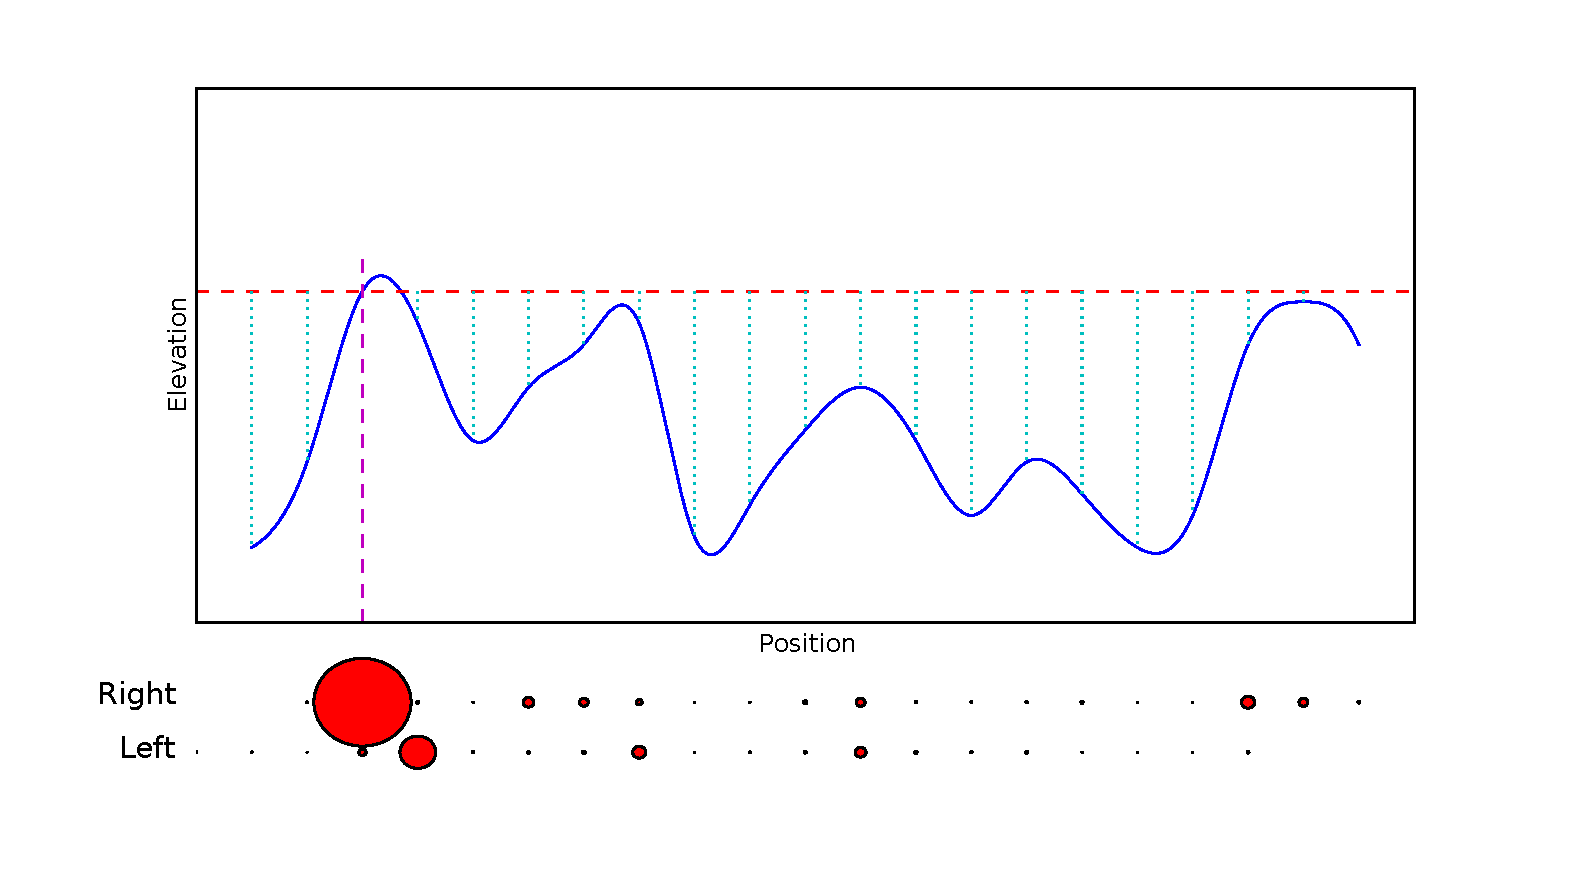
\includegraphics[width=\textwidth]{meas2}\\
\note{
\begin{itemize}
    \item So the true location now how been correct twice in a row.
    \item Note that traveling left over the hill results in similar 
            measurements
\end{itemize}
}
\end{frame}

\begin{frame}{Step Forward}
\centering
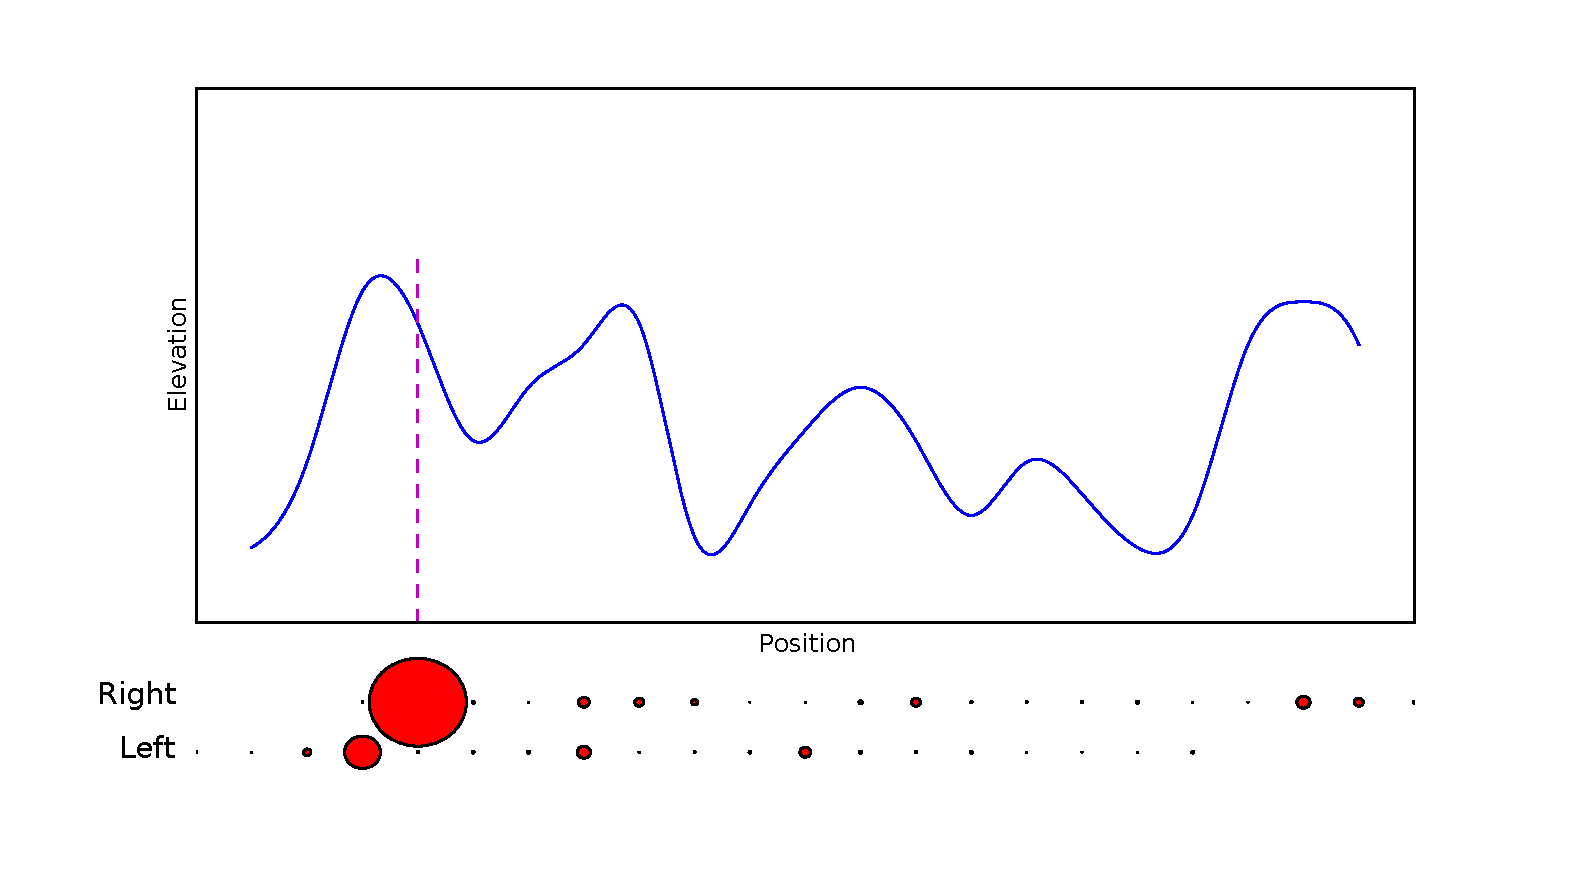
\includegraphics[width=\textwidth]{move2}\\
\end{frame}

\begin{frame}{Particle Filter Concepts}
\small
\begin{columns}
\begin{column}{.5\textwidth}
\begin{itemize}
    \item Weighting Function
        \begin{itemize}
            \item Converts Discrete Estimates of $y$ 
                    Into a Continuous Estimate of $y$
        \end{itemize}
    \item Particle Density
    \item Resampling
    \begin{itemize}
        \item Remove Useless Particles
    \end{itemize}
    \item Regularized Resampling
    \begin{itemize}
        \item Prevent Identical Particles
    \end{itemize}
\end{itemize}
\end{column}

\begin{column}{.5\textwidth}
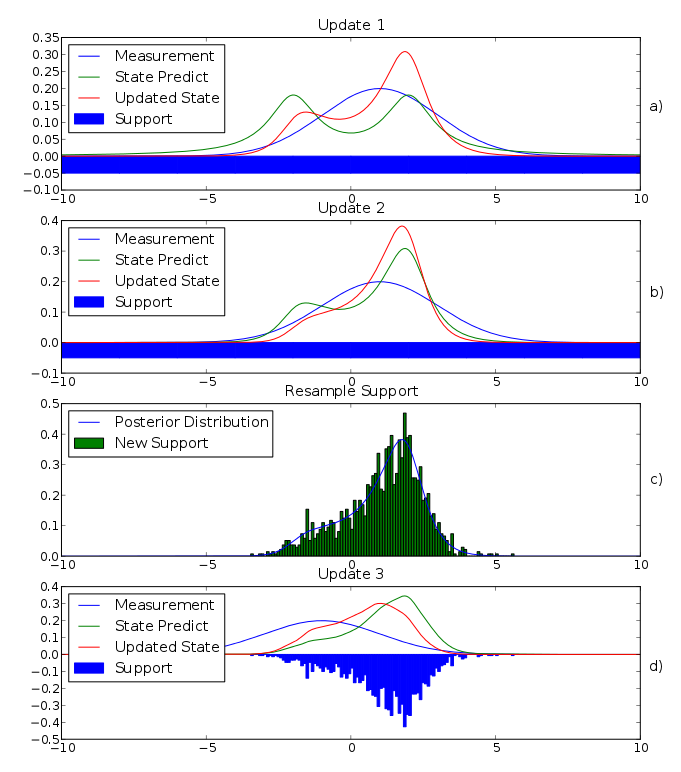
\includegraphics[clip=true,trim=.75cm 7.07cm .5cm 7cm,width=\textwidth]{particle_filter2}
\end{column}
\end{columns}
\note{
    \tiny
\begin{itemize}
    \item Weighting function decides how much you want to weight particles
            that don't exactly match the measurement
    \item The weighting function and the particle density 
            (distance between particles) form a sort of net
    \item Whether the net has holes also depends on the maximum gradient
            of $y$ with respect to the parameters
    \item Resampling allows the algorithm to increase density in areas
            of interest. 
    \item Resampling could also remove "good" areas
    \item Resampling typically draws from the set of existing particles,
            reducing the number of unique particles
    \item Regularized resampling, instead draws from a smooth version of
            the posterior distribution, so particles are always unique
\end{itemize}
}
\end{frame}

\begin{frame}{Particle Construction, Particle $i$, Time $k$}
\begin{columns}
\begin{column}{.54\textwidth}
\begin{itemize}
    \item Mixture PDF, with $N_p$ particles:
        $$P(x_k) = \sum_{i=0}^{N_p} w_k^i\delta(x_k - x^i_k )$$
    \item Weight Definition:
        $$w^i_k \propto \frac{P(x^i_{0:k} | y_{0:k})}{q(x^i_{0:k} | y_{0:k})}$$
    \item Incorporating Measurement $y_k$:
        $$w^i_k \propto & w^i_{k-1}P(y_k| x^i_k) $$
\end{itemize}
\end{column}

\begin{column}{.46\textwidth}
\tiny
\ifx\du\undefined
  \newlength{\du}
\fi
\setlength{\du}{10\unitlength}
\begin{tikzpicture}
\pgftransformxscale{1.000000}
\pgftransformyscale{-1.000000}
\definecolor{dialinecolor}{rgb}{0.000000, 0.000000, 0.000000}
\pgfsetstrokecolor{dialinecolor}
\definecolor{dialinecolor}{rgb}{1.000000, 1.000000, 1.000000}
\pgfsetfillcolor{dialinecolor}
\pgfsetlinewidth{0.050000\du}
\pgfsetdash{}{0pt}
\definecolor{dialinecolor}{rgb}{1.000000, 1.000000, 1.000000}
\pgfsetfillcolor{dialinecolor}
\fill (9.250000\du,3.650000\du)--(9.250000\du,5.050000\du)--(12.1000\du,5.050000\du)--(12.1000\du,3.650000\du)--cycle;
\definecolor{dialinecolor}{rgb}{0.000000, 0.000000, 0.000000}
\pgfsetstrokecolor{dialinecolor}
\draw (9.250000\du,3.650000\du)--(9.250000\du,5.050000\du)--(12.1000\du,5.050000\du)--(12.1000\du,3.650000\du)--cycle;
% setfont left to latex
\definecolor{dialinecolor}{rgb}{0.000000, 0.000000, 0.000000}
\pgfsetstrokecolor{dialinecolor}
\node at (10.732500\du,4.600000\du){Particle};
\definecolor{dialinecolor}{rgb}{1.000000, 1.000000, 1.000000}
\pgfsetfillcolor{dialinecolor}
\fill (9.250000\du,5.050000\du)--(9.250000\du,14.050000\du)--(12.1000\du,14.050000\du)--(12.1000\du,5.050000\du)--cycle;
\definecolor{dialinecolor}{rgb}{0.000000, 0.000000, 0.000000}
\pgfsetstrokecolor{dialinecolor}
\draw (9.250000\du,5.050000\du)--(9.250000\du,14.050000\du)--(12.1000\du,14.050000\du)--(12.1000\du,5.050000\du)--cycle;
% setfont left to latex
\definecolor{dialinecolor}{rgb}{0.000000, 0.000000, 0.000000}
\pgfsetstrokecolor{dialinecolor}
\node[anchor=west] at (9.400000\du,5.750000\du){\color{mblue} $s$};
% setfont left to latex
\definecolor{dialinecolor}{rgb}{0.000000, 0.000000, 0.000000}
\pgfsetstrokecolor{dialinecolor}
\node[anchor=west] at (9.400000\du,6.550000\du){\color{mblue} $f$};
% setfont left to latex
\definecolor{dialinecolor}{rgb}{0.000000, 0.000000, 0.000000}
\pgfsetstrokecolor{dialinecolor}
\node[anchor=west] at (9.400000\du,7.350000\du){\color{mblue} $q$};
% setfont left to latex
\definecolor{dialinecolor}{rgb}{0.000000, 0.000000, 0.000000}
\pgfsetstrokecolor{dialinecolor}
\node[anchor=west] at (9.400000\du,8.150000\du){\color{mblue} $v$};
% setfont left to latex
\definecolor{dialinecolor}{rgb}{0.000000, 0.000000, 0.000000}
\pgfsetstrokecolor{dialinecolor}
\node[anchor=west] at (9.400000\du,8.950000\du){\color{mred} $\epsilon$};
% setfont left to latex
\definecolor{dialinecolor}{rgb}{0.000000, 0.000000, 0.000000}
\pgfsetstrokecolor{dialinecolor}
\node[anchor=west] at (9.400000\du,9.750000\du){\color{mred} $\tau_f$};
% setfont left to latex
\definecolor{dialinecolor}{rgb}{0.000000, 0.000000, 0.000000}
\pgfsetstrokecolor{dialinecolor}
\node[anchor=west] at (9.400000\du,10.550000\du){\color{mred} $\tau_s$};
% setfont left to latex
\definecolor{dialinecolor}{rgb}{0.000000, 0.000000, 0.000000}
\pgfsetstrokecolor{dialinecolor}
\node[anchor=west] at (9.400000\du,11.350000\du){\color{mred} $\tau_0$};
% setfont left to latex
\definecolor{dialinecolor}{rgb}{0.000000, 0.000000, 0.000000}
\pgfsetstrokecolor{dialinecolor}
\node[anchor=west] at (9.400000\du,12.150000\du){\color{mred} $\alpha$};
% setfont left to latex
\definecolor{dialinecolor}{rgb}{0.000000, 0.000000, 0.000000}
\pgfsetstrokecolor{dialinecolor}
\node[anchor=west] at (9.400000\du,12.950000\du){\color{mred} $E_0$};
% setfont left to latex
\definecolor{dialinecolor}{rgb}{0.000000, 0.000000, 0.000000}
\pgfsetstrokecolor{dialinecolor}
\node[anchor=west] at (9.400000\du,13.750000\du){\color{mred} $V_0$};
\definecolor{dialinecolor}{rgb}{1.000000, 1.000000, 1.000000}
\pgfsetfillcolor{dialinecolor}
\fill (9.250000\du,14.050000\du)--(9.250000\du,15.050000\du)--(12.1000\du,15.050000\du)--(12.1000\du,14.050000\du)--cycle;
\definecolor{dialinecolor}{rgb}{0.000000, 0.000000, 0.000000}
\pgfsetstrokecolor{dialinecolor}
\draw (9.250000\du,14.050000\du)--(9.250000\du,15.050000\du)--(12.1000\du,15.050000\du)--(12.1000\du,14.050000\du)--cycle;
% setfont left to latex
\definecolor{dialinecolor}{rgb}{0.000000, 0.000000, 0.000000}
\pgfsetstrokecolor{dialinecolor}
\node[anchor=west] at (9.400000\du,14.750000\du){ weight};
% setfont left to latex
\definecolor{dialinecolor}{rgb}{0.000000, 0.000000, 0.000000}
\pgfsetstrokecolor{dialinecolor}
\node[anchor=west] at (5.050000\du,5.850000\du){};
% setfont left to latex
\definecolor{dialinecolor}{rgb}{0.000000, 0.000000, 0.000000}
\pgfsetstrokecolor{dialinecolor}
\node[anchor=west] at (5.100000\du,6.500000\du){Change};
% setfont left to latex
\definecolor{dialinecolor}{rgb}{0.000000, 0.000000, 0.000000}
\pgfsetstrokecolor{dialinecolor}
\node[anchor=west] at (5.100000\du,7.300000\du){With Time};
% setfont left to latex
\definecolor{dialinecolor}{rgb}{0.000000, 0.000000, 0.000000}
\pgfsetstrokecolor{dialinecolor}
\node[anchor=west] at (13.000000\du,9.850000\du){Change When};
% setfont left to latex
\definecolor{dialinecolor}{rgb}{0.000000, 0.000000, 0.000000}
\pgfsetstrokecolor{dialinecolor}
\node[anchor=west] at (13.000000\du,10.650000\du){Resampling};
\pgfsetlinewidth{0.050000\du}
\pgfsetdash{}{0pt}
\pgfsetdash{}{0pt}
\pgfsetbuttcap
{
\definecolor{dialinecolor}{rgb}{0.000000, 0.000000, 0.000000}
\pgfsetfillcolor{dialinecolor}
% was here!!!
\definecolor{dialinecolor}{rgb}{0.000000, 0.000000, 0.000000}
\pgfsetstrokecolor{dialinecolor}
\pgfpathmoveto{\pgfpoint{9.000025\du}{5.399967\du}}
\pgfpatharc{217}{144}{1.000000\du and 1.000000\du}
\pgfusepath{stroke}
}
\pgfsetlinewidth{0.050000\du}
\pgfsetdash{}{0pt}
\pgfsetdash{}{0pt}
\pgfsetbuttcap
{
\definecolor{dialinecolor}{rgb}{0.000000, 0.000000, 0.000000}
\pgfsetfillcolor{dialinecolor}
% was here!!!
\definecolor{dialinecolor}{rgb}{0.000000, 0.000000, 0.000000}
\pgfsetstrokecolor{dialinecolor}
\pgfpathmoveto{\pgfpoint{9.000025\du}{6.999967\du}}
\pgfpatharc{217}{144}{1.000000\du and 1.000000\du}
\pgfusepath{stroke}
}
\pgfsetlinewidth{0.050000\du}
\pgfsetdash{}{0pt}
\pgfsetdash{}{0pt}
\pgfsetbuttcap
{
\definecolor{dialinecolor}{rgb}{0.000000, 0.000000, 0.000000}
\pgfsetfillcolor{dialinecolor}
% was here!!!
\definecolor{dialinecolor}{rgb}{0.000000, 0.000000, 0.000000}
\pgfsetstrokecolor{dialinecolor}
\draw (9.000000\du,6.600000\du)--(8.600000\du,6.800000\du);
}
\pgfsetlinewidth{0.050000\du}
\pgfsetdash{}{0pt}
\pgfsetdash{}{0pt}
\pgfsetbuttcap
{
\definecolor{dialinecolor}{rgb}{0.000000, 0.000000, 0.000000}
\pgfsetfillcolor{dialinecolor}
% was here!!!
\definecolor{dialinecolor}{rgb}{0.000000, 0.000000, 0.000000}
\pgfsetstrokecolor{dialinecolor}
\draw (8.600000\du,6.800000\du)--(9.000000\du,7.000000\du);
}
\pgfsetlinewidth{0.050000\du}
\pgfsetdash{}{0pt}
\pgfsetdash{}{0pt}
\pgfsetbuttcap
{
\definecolor{dialinecolor}{rgb}{0.000000, 0.000000, 0.000000}
\pgfsetfillcolor{dialinecolor}
% was here!!!
\definecolor{dialinecolor}{rgb}{0.000000, 0.000000, 0.000000}
\pgfsetstrokecolor{dialinecolor}
\pgfpathmoveto{\pgfpoint{12.399753\du}{9.80\du}}
\pgfpatharc{10}{-9}{12.965299\du and 12.965299\du}
\pgfusepath{stroke}
}
\pgfsetlinewidth{0.050000\du}
\pgfsetdash{}{0pt}
\pgfsetdash{}{0pt}
\pgfsetbuttcap
{
\definecolor{dialinecolor}{rgb}{0.000000, 0.000000, 0.000000}
\pgfsetfillcolor{dialinecolor}
% was here!!!
\definecolor{dialinecolor}{rgb}{0.000000, 0.000000, 0.000000}
\pgfsetstrokecolor{dialinecolor}
\pgfpathmoveto{\pgfpoint{12.419203\du}{15.0\du}}
\pgfpatharc{10}{-9}{12.847799\du and 12.847799\du}
\pgfusepath{stroke}
}
\pgfsetlinewidth{0.050000\du}
\pgfsetdash{}{0pt}
\pgfsetdash{}{0pt}
\pgfsetbuttcap
{
\definecolor{dialinecolor}{rgb}{0.000000, 0.000000, 0.000000}
\pgfsetfillcolor{dialinecolor}
% was here!!!
\definecolor{dialinecolor}{rgb}{0.000000, 0.000000, 0.000000}
\pgfsetstrokecolor{dialinecolor}
\draw (12.400000\du,9.800000\du)--(13.019438\du,10.220000\du);
}
\pgfsetlinewidth{0.050000\du}
\pgfsetdash{}{0pt}
\pgfsetdash{}{0pt}
\pgfsetbuttcap
{
\definecolor{dialinecolor}{rgb}{0.000000, 0.000000, 0.000000}
\pgfsetfillcolor{dialinecolor}
% was here!!!
\definecolor{dialinecolor}{rgb}{0.000000, 0.000000, 0.000000}
\pgfsetstrokecolor{dialinecolor}
\draw (13.019438\du,10.220000\du)--(12.440000\du,10.760000\du);
}
% setfont left to latex
\definecolor{dialinecolor}{rgb}{0.000000, 0.000000, 0.000000}
\pgfsetstrokecolor{dialinecolor}
\node[anchor=west] at (4.000000\du,15.000000\du){Change When};
% setfont left to latex
\definecolor{dialinecolor}{rgb}{0.000000, 0.000000, 0.000000}
\pgfsetstrokecolor{dialinecolor}
\node[anchor=west] at (4.000000\du,15.800000\du){Incorporating Measurement};
\pgfsetlinewidth{0.050000\du}
\pgfsetdash{}{0pt}
\pgfsetdash{}{0pt}
\pgfsetbuttcap
{
\definecolor{dialinecolor}{rgb}{0.000000, 0.000000, 0.000000}
\pgfsetfillcolor{dialinecolor}
% was here!!!
\definecolor{dialinecolor}{rgb}{0.000000, 0.000000, 0.000000}
\pgfsetstrokecolor{dialinecolor}
\draw (9.000000\du,14.200000\du)--(8.600000\du,14.800000\du);
}
\pgfsetlinewidth{0.050000\du}
\pgfsetdash{}{0pt}
\pgfsetdash{}{0pt}
\pgfsetbuttcap
{
\definecolor{dialinecolor}{rgb}{0.000000, 0.000000, 0.000000}
\pgfsetfillcolor{dialinecolor}
% was here!!!
\definecolor{dialinecolor}{rgb}{0.000000, 0.000000, 0.000000}
\pgfsetstrokecolor{dialinecolor}
\draw (9.000000\du,15.000000\du)--(8.600000\du,14.800000\du);
}
\end{tikzpicture}

\end{column}
\end{columns}
\note{
    \tiny
    \begin{itemize}
        \item The posterior distribution is represented by a mixture
                PDF, where the probability of a discrete point is based
                on its relative weight.
        \item The definition of the weight function is given. 
        \item $q$ is the importance density, which is just the location
            of the particles. When you plug in the weights, that 
            term and the $\delta$ cancel and you are just left
            with the probability of getting that timeseries of 
            states given the timeseries of measurements.
        \item After some simplification, it comes out that weights
            can be updated with new measurements rather simply.
        \item On the right that each particle has an estimate
            for all of those states and unknown parameters.
        \item Weights Don't Integrate to 1.

    \end{itemize}
}
\end{frame}

%\ifx\du\undefined
%  \newlength{\du}
%\fi
%\setlength{\du}{10\unitlength}
%\begin{tikzpicture}
%\pgftransformxscale{1.000000}
%\pgftransformyscale{-1.000000}
%\definecolor{dialinecolor}{rgb}{0.000000, 0.000000, 0.000000}
%\pgfsetstrokecolor{dialinecolor}
%\definecolor{dialinecolor}{rgb}{1.000000, 1.000000, 1.000000}
%\pgfsetfillcolor{dialinecolor}
%\pgfsetlinewidth{0.050000\du}
%\pgfsetdash{}{0pt}
%\definecolor{dialinecolor}{rgb}{1.000000, 1.000000, 1.000000}
%\pgfsetfillcolor{dialinecolor}
%\fill (9.250000\du,3.650000\du)--(9.250000\du,5.050000\du)--(13.215000\du,5.050000\du)--(13.215000\du,3.650000\du)--cycle;
%\definecolor{dialinecolor}{rgb}{0.000000, 0.000000, 0.000000}
%\pgfsetstrokecolor{dialinecolor}
%\draw (9.250000\du,3.650000\du)--(9.250000\du,5.050000\du)--(13.215000\du,5.050000\du)--(13.215000\du,3.650000\du)--cycle;
%% setfont left to latex
%\definecolor{dialinecolor}{rgb}{0.000000, 0.000000, 0.000000}
%\pgfsetstrokecolor{dialinecolor}
%\node at (11.232500\du,4.600000\du){Particle};
%\definecolor{dialinecolor}{rgb}{1.000000, 1.000000, 1.000000}
%\pgfsetfillcolor{dialinecolor}
%\fill (9.250000\du,5.050000\du)--(9.250000\du,14.050000\du)--(13.215000\du,14.050000\du)--(13.215000\du,5.050000\du)--cycle;
%\definecolor{dialinecolor}{rgb}{0.000000, 0.000000, 0.000000}
%\pgfsetstrokecolor{dialinecolor}
%\draw (9.250000\du,5.050000\du)--(9.250000\du,14.050000\du)--(13.215000\du,14.050000\du)--(13.215000\du,5.050000\du)--cycle;
%% setfont left to latex
%\definecolor{dialinecolor}{rgb}{0.000000, 0.000000, 0.000000}
%\pgfsetstrokecolor{dialinecolor}
%\node[anchor=west] at (9.400000\du,5.750000\du){\color{mblue} $s$};
%% setfont left to latex
%\definecolor{dialinecolor}{rgb}{0.000000, 0.000000, 0.000000}
%\pgfsetstrokecolor{dialinecolor}
%\node[anchor=west] at (9.400000\du,6.550000\du){\color{mblue} $f$};
%% setfont left to latex
%\definecolor{dialinecolor}{rgb}{0.000000, 0.000000, 0.000000}
%\pgfsetstrokecolor{dialinecolor}
%\node[anchor=west] at (9.400000\du,7.350000\du){\color{mblue} $q$};
%% setfont left to latex
%\definecolor{dialinecolor}{rgb}{0.000000, 0.000000, 0.000000}
%\pgfsetstrokecolor{dialinecolor}
%\node[anchor=west] at (9.400000\du,8.150000\du){\color{mblue} $v$};
%% setfont left to latex
%\definecolor{dialinecolor}{rgb}{0.000000, 0.000000, 0.000000}
%\pgfsetstrokecolor{dialinecolor}
%\node[anchor=west] at (9.400000\du,8.950000\du){\color{mred} $\epsilon$};
%% setfont left to latex
%\definecolor{dialinecolor}{rgb}{0.000000, 0.000000, 0.000000}
%\pgfsetstrokecolor{dialinecolor}
%\node[anchor=west] at (9.400000\du,9.750000\du){\color{mred} $\tau_f$};
%% setfont left to latex
%\definecolor{dialinecolor}{rgb}{0.000000, 0.000000, 0.000000}
%\pgfsetstrokecolor{dialinecolor}
%\node[anchor=west] at (9.400000\du,10.550000\du){\color{mred} $\tau_s$};
%% setfont left to latex
%\definecolor{dialinecolor}{rgb}{0.000000, 0.000000, 0.000000}
%\pgfsetstrokecolor{dialinecolor}
%\node[anchor=west] at (9.400000\du,11.350000\du){\color{mred} $\tau_0$};
%% setfont left to latex
%\definecolor{dialinecolor}{rgb}{0.000000, 0.000000, 0.000000}
%\pgfsetstrokecolor{dialinecolor}
%\node[anchor=west] at (9.400000\du,12.150000\du){\color{mred} $\alpha$};
%% setfont left to latex
%\definecolor{dialinecolor}{rgb}{0.000000, 0.000000, 0.000000}
%\pgfsetstrokecolor{dialinecolor}
%\node[anchor=west] at (9.400000\du,12.950000\du){\color{mred} $\E_0$};
%% setfont left to latex
%\definecolor{dialinecolor}{rgb}{0.000000, 0.000000, 0.000000}
%\pgfsetstrokecolor{dialinecolor}
%\node[anchor=west] at (9.400000\du,13.750000\du){\color{mred} $V_0$};
%\definecolor{dialinecolor}{rgb}{1.000000, 1.000000, 1.000000}
%\pgfsetfillcolor{dialinecolor}
%\fill (9.250000\du,14.050000\du)--(9.250000\du,15.050000\du)--(13.215000\du,15.050000\du)--(13.215000\du,14.050000\du)--cycle;
%\definecolor{dialinecolor}{rgb}{0.000000, 0.000000, 0.000000}
%\pgfsetstrokecolor{dialinecolor}
%\draw (9.250000\du,14.050000\du)--(9.250000\du,15.050000\du)--(13.215000\du,15.050000\du)--(13.215000\du,14.050000\du)--cycle;
%% setfont left to latex
%\definecolor{dialinecolor}{rgb}{0.000000, 0.000000, 0.000000}
%\pgfsetstrokecolor{dialinecolor}
%\node[anchor=west] at (9.400000\du,14.750000\du){weight};
%% setfont left to latex
%\definecolor{dialinecolor}{rgb}{0.000000, 0.000000, 0.000000}
%\pgfsetstrokecolor{dialinecolor}
%\node[anchor=west] at (5.050000\du,5.850000\du){};
%% setfont left to latex
%\definecolor{dialinecolor}{rgb}{0.000000, 0.000000, 0.000000}
%\pgfsetstrokecolor{dialinecolor}
%\node[anchor=west] at (5.100000\du,6.500000\du){Change};
%% setfont left to latex
%\definecolor{dialinecolor}{rgb}{0.000000, 0.000000, 0.000000}
%\pgfsetstrokecolor{dialinecolor}
%\node[anchor=west] at (5.100000\du,7.300000\du){With Time};
%% setfont left to latex
%\definecolor{dialinecolor}{rgb}{0.000000, 0.000000, 0.000000}
%\pgfsetstrokecolor{dialinecolor}
%\node[anchor=west] at (14.450000\du,9.850000\du){Change When};
%% setfont left to latex
%\definecolor{dialinecolor}{rgb}{0.000000, 0.000000, 0.000000}
%\pgfsetstrokecolor{dialinecolor}
%\node[anchor=west] at (14.450000\du,10.650000\du){Resampling};
%\pgfsetlinewidth{0.050000\du}
%\pgfsetdash{}{0pt}
%\pgfsetdash{}{0pt}
%\pgfsetbuttcap
%{
%\definecolor{dialinecolor}{rgb}{0.000000, 0.000000, 0.000000}
%\pgfsetfillcolor{dialinecolor}
%% was here!!!
%\definecolor{dialinecolor}{rgb}{0.000000, 0.000000, 0.000000}
%\pgfsetstrokecolor{dialinecolor}
%\pgfpathmoveto{\pgfpoint{9.000025\du}{5.399967\du}}
%\pgfpatharc{217}{144}{1.000000\du and 1.000000\du}
%\pgfusepath{stroke}
%}
%\pgfsetlinewidth{0.050000\du}
%\pgfsetdash{}{0pt}
%\pgfsetdash{}{0pt}
%\pgfsetbuttcap
%{
%\definecolor{dialinecolor}{rgb}{0.000000, 0.000000, 0.000000}
%\pgfsetfillcolor{dialinecolor}
%% was here!!!
%\definecolor{dialinecolor}{rgb}{0.000000, 0.000000, 0.000000}
%\pgfsetstrokecolor{dialinecolor}
%\pgfpathmoveto{\pgfpoint{9.000025\du}{6.999967\du}}
%\pgfpatharc{217}{144}{1.000000\du and 1.000000\du}
%\pgfusepath{stroke}
%}
%\pgfsetlinewidth{0.050000\du}
%\pgfsetdash{}{0pt}
%\pgfsetdash{}{0pt}
%\pgfsetbuttcap
%{
%\definecolor{dialinecolor}{rgb}{0.000000, 0.000000, 0.000000}
%\pgfsetfillcolor{dialinecolor}
%% was here!!!
%\definecolor{dialinecolor}{rgb}{0.000000, 0.000000, 0.000000}
%\pgfsetstrokecolor{dialinecolor}
%\draw (9.000000\du,6.600000\du)--(8.600000\du,6.800000\du);
%}
%\pgfsetlinewidth{0.050000\du}
%\pgfsetdash{}{0pt}
%\pgfsetdash{}{0pt}
%\pgfsetbuttcap
%{
%\definecolor{dialinecolor}{rgb}{0.000000, 0.000000, 0.000000}
%\pgfsetfillcolor{dialinecolor}
%% was here!!!
%\definecolor{dialinecolor}{rgb}{0.000000, 0.000000, 0.000000}
%\pgfsetstrokecolor{dialinecolor}
%\draw (8.600000\du,6.800000\du)--(9.000000\du,7.000000\du);
%}
%\pgfsetlinewidth{0.050000\du}
%\pgfsetdash{}{0pt}
%\pgfsetdash{}{0pt}
%\pgfsetbuttcap
%{
%\definecolor{dialinecolor}{rgb}{0.000000, 0.000000, 0.000000}
%\pgfsetfillcolor{dialinecolor}
%% was here!!!
%\definecolor{dialinecolor}{rgb}{0.000000, 0.000000, 0.000000}
%\pgfsetstrokecolor{dialinecolor}
%\pgfpathmoveto{\pgfpoint{13.419202\du}{9.691344\du}}
%\pgfpatharc{10}{-9}{13.325000\du and 13.325000\du}
%\pgfusepath{stroke}
%}
%\pgfsetlinewidth{0.050000\du}
%\pgfsetdash{}{0pt}
%\pgfsetdash{}{0pt}
%\pgfsetbuttcap
%{
%\definecolor{dialinecolor}{rgb}{0.000000, 0.000000, 0.000000}
%\pgfsetfillcolor{dialinecolor}
%% was here!!!
%\definecolor{dialinecolor}{rgb}{0.000000, 0.000000, 0.000000}
%\pgfsetstrokecolor{dialinecolor}
%\pgfpathmoveto{\pgfpoint{13.419202\du}{15.091344\du}}
%\pgfpatharc{10}{-9}{13.325000\du and 13.325000\du}
%\pgfusepath{stroke}
%}
%\pgfsetlinewidth{0.050000\du}
%\pgfsetdash{}{0pt}
%\pgfsetdash{}{0pt}
%\pgfsetbuttcap
%{
%\definecolor{dialinecolor}{rgb}{0.000000, 0.000000, 0.000000}
%\pgfsetfillcolor{dialinecolor}
%% was here!!!
%\definecolor{dialinecolor}{rgb}{0.000000, 0.000000, 0.000000}
%\pgfsetstrokecolor{dialinecolor}
%\draw (13.419438\du,9.690000\du)--(14.019438\du,10.090000\du);
%}
%\pgfsetlinewidth{0.050000\du}
%\pgfsetdash{}{0pt}
%\pgfsetdash{}{0pt}
%\pgfsetbuttcap
%{
%\definecolor{dialinecolor}{rgb}{0.000000, 0.000000, 0.000000}
%\pgfsetfillcolor{dialinecolor}
%% was here!!!
%\definecolor{dialinecolor}{rgb}{0.000000, 0.000000, 0.000000}
%\pgfsetstrokecolor{dialinecolor}
%#\draw (14.019438\du,10.090000\du)--(13.419438\du,10.490000\du);
%}
%\pgfsetlinewidth{0.050000\du}
%\pgfsetdash{}{0pt}
%\pgfsetdash{}{0pt}
%\pgfsetbuttcap
%{
%\definecolor{dialinecolor}{rgb}{0.000000, 0.000000, 0.000000}
%\pgfsetfillcolor{dialinecolor}
%% was here!!!
%\definecolor{dialinecolor}{rgb}{0.000000, 0.000000, 0.000000}
%\pgfsetstrokecolor{dialinecolor}
%\pgfpathmoveto{\pgfpoint{9.000021\du}{13.999975\du}}
%\pgfpatharc{219}{136}{0.790625\du and 0.790625\du}
%\pgfusepath{stroke}
%}
%% setfont left to latex
%\definecolor{dialinecolor}{rgb}{0.000000, 0.000000, 0.000000}
%\pgfsetstrokecolor{dialinecolor}
%\node[anchor=west] at (4.000000\du,15.000000\du){Change When};
%% setfont left to latex
%\definecolor{dialinecolor}{rgb}{0.000000, 0.000000, 0.000000}
%\pgfsetstrokecolor{dialinecolor}
%\node[anchor=west] at (4.000000\du,15.800000\du){Adding Measurement};
%\end{tikzpicture}
